\chapter{Erweiterung durch eine Siri Integration}
Johannes Franz \& Normen Krug

\section{Einleitung}
Da sprachbasierte Mensch-Maschinen-Interface immer beliebter und praktikabler werden, ist es naheliegend, dass die Stundenplan App um diese erweitert wird. Apple bietet mit Siri solch einen Sprachassistenten ein. Dieser ist tief im System eingebaut und wird daher von Apple gut unterstützt. 
Da es weiterhin das Ziel sein soll, die App zur Nutzung nicht öffnen zu müssen, ist eine Siri Integration der nächst logische Schritt zur Weiterentwicklung der Anwendung.

\begin{figure}[H]
	\centering
  \frame{ 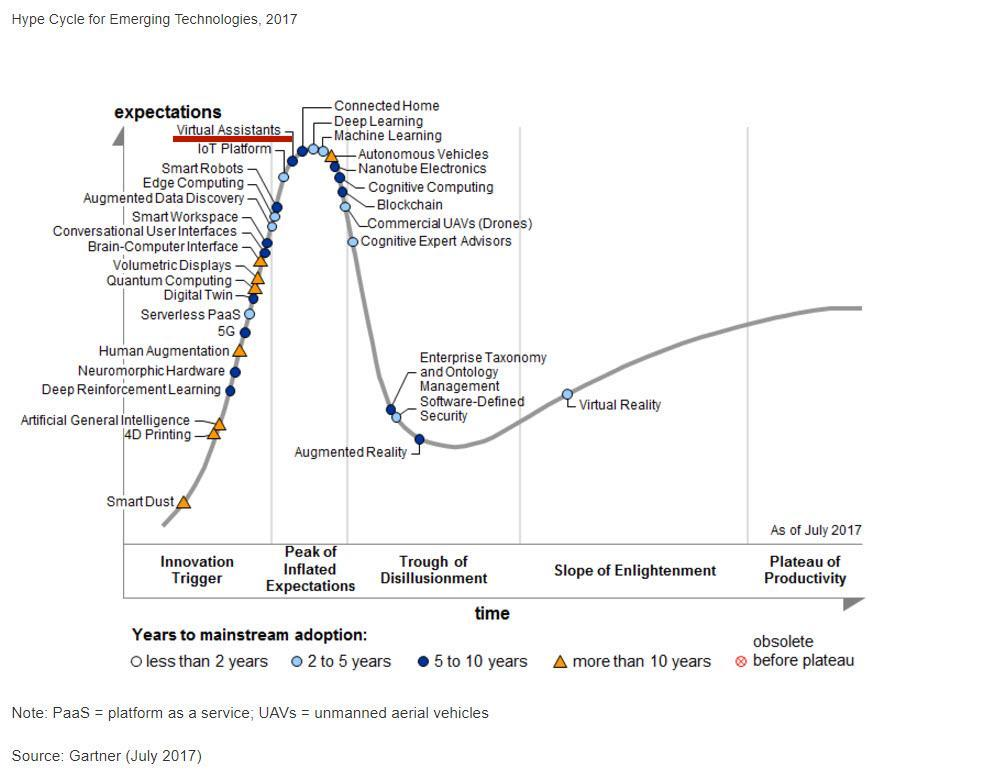
\includegraphics[width=0.9\textwidth]{hype-cycle-for-emerging-technologies-2017} }
	\caption{hype cycle for technologies 2017}
	\label{hype}
\end{figure}


\section{Istzustand}
Die App bietet aktuell keine Unterstützung für Sprachbefehle an. Eine Eingabe durch Sprachbefehle durch die Apple Watch ist so ebenfalls nicht möglich. Im Hinblick auf barrierefreie Bedienung hat die App daher noch Verbesserungspotential.

\section{Beispielhafte Anfragen}
Um die gängigen Anfragen abzudecken, müssen diese in der App vorher festgelegt werden. Um das Anliegen des Benutzers verstehen zu können müssen unterschiedliche Fragestellungen die zum selben Ergebnis führen abgedeckt werden.


\noindent%
\begin{tabularx}{\textwidth}{|p{.25\textwidth}|X| }
\hline
\textbf{Frage} & \textbf{Reaktion}  \\ \hline 

Wann/Wo ist meine nächste Vorlesung? & Name der Vorlesung, Zeitspanne und Raumnummer vorlesen.
UI zeigt diese Information noch einmal an.\\ \hline

Habe ich heute noch eine Vorlesung? & Ja/Nein Antwort, Name der Vorlesung mit Uhrzeit. 
Wenn ja wird im UI etwas angezeigt.
\\ \hline

Fällt heute etwas aus? & Ja/Nein Antwort, Name der Vorlesung mit Uhrzeit mit Grund. 
Wenn ja wird im UI etwas angezeigt.\\ \hline
Welche Änderungen gibt es heute? & Aufzählung der Änderungen für heute.
Auflisten dieser Änderungen im UI\\ \hline
In welchem Raum ist Vorlesung X? (optional/tricky) & Name der Vorlesung und Raum wird genannt.
Informationen im UI werden angezeigt.
\\ \hline

\end{tabularx}

\section{Umsetzung}
Apple bietet für die Umsetzung des Sprachassistenten das SiriKit an. Mittels einer “Applications Extension” namens “Intents Extension” ist es möglich Hooks für eine Reaktion der Stundenplan App zu definieren. Für die Ausgabe im Lockscreen kann dabei ein angepasstes UI zur Verfügung gestellt werden, welches die Sprachausgabe ergänzt.
\newline


\begin{figure}[H]
	\centering
  \frame{ 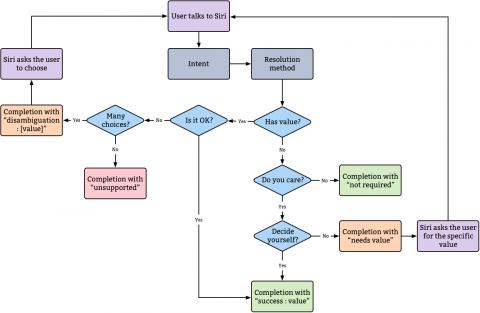
\includegraphics[width=0.9\textwidth]{Siri_Flowchart} }
	\caption{Siri Flowchart}
	\label{flowchart}
\end{figure}


\section{Voraussetzung für SiriKit}

Stand: 10.10.2017

Um SiriKit verwenden zu können, müssen die Kernbereiche der App in ein Framework ausgelagert werden. 
Apple empfiehlt das bei allen Erweiterungen.  Dieser Schritt ist notwendig, weil der Benutzer eine Interaktion mit Siri starten kann auch wenn die App zurzeit nicht läuft.  



\section{Einschränkungen}

Apple gewährt keinen vollständigen Zugriff auf Siri. Die zu entwickelte App muss in eine der Folgenden Kategorien/Domains fallen:
%\newline
\begin{itemize}
\item VoIP Calling 
\item Messaging
\item Payments
\item Lists and Notes
\item Visual Codes
\item Photos
\item Workouts
\item Ride Booking
\item Car Commands
\item CarPlay
\item Restaurant Reservations
\end{itemize}

\newpage

Die Schlüsselwörter welche Siri voraussetzt, um zu erkennen dass der Benutzer mit der App interagieren will, hängen von der Domain ab.
Diese Schlüsselwörter müssen zwingend in der Anfrage des Benutzer enthalten sein. 

Beispiel: 

In der „Search Message“  Domain müssen die Wörter „Suche“ und „Nachrichten“ enthalten sein. Falls eines der beiden Wörter nicht in der Anfrage enthalten ist, erkennt Siri die Anfrage nicht.  \newline
Passender Blog-Post zu den Thema: \newline
\url{https://swifting.io/blog/2016/07/18/20-sirikit-can-you-outsmart-provided-intents/}

Mögliche Workarounds: \newline
Es ist theoretisch möglichen mit der „Lists and Notes“ Domain, die Funktion für die Stundenplan hinzubiegen. Da aber die bestimmten Schlüsselwörter enthalten sei müssen, wird aber kein natürlich sprachliche Interaktion möglich sein.
\url{https://developer.apple.com/documentation/sirikit}

\section{Fazit}
Die vielversprechenden Idee die App um einen Sprachassistenten zu erweitern, ist zum aktuellen Zeitpunkt nicht realisierbar aufgrund der Limitierunegn vom SiriKit. Das Projekt musste an dieser Stelle unterbrochen werden und das Team musste sich neu orientieren.\\
Da Apple den Sprachassistenten Siri stets erweitert, kann allerdings darauf gehofft werden, dass einer Umsetzung zu einem späteren Zeitpunkt keine Barrieren mehr im Wege stehen.